\documentclass[11pt,oneside]{report} 

\usepackage{ stmaryrd }
\usepackage{cite}
\usepackage{graphicx}
\usepackage[utf8]{inputenc}
\usepackage[T1]{fontenc}
\usepackage[spanish]{babel}
\usepackage{csquotes}
\usepackage{graphicx}
\usepackage{listings}
\usepackage{xcolor}
\usepackage{hyperref}
\usepackage{geometry}
\usepackage{tikz}
\usetikzlibrary{shapes,arrows}
\usetikzlibrary{positioning}
\setlength{\parindent}{0.5in}
\usepackage{setspace}
\usepackage{amssymb}
\usepackage{amsthm}
\usepackage{ dsfont }
\usepackage{amsmath,amsfonts,amssymb}
\usepackage{ragged2e}
\hypersetup{
    colorlinks=true,
    linkcolor=black,
    filecolor=magenta,      
    urlcolor=gray,
}

\renewcommand{\baselinestretch}{1.5}

\theoremstyle{plain}
\newtheorem{proposición}{proposición}[chapter] 
\newtheorem{lema}{Lema}[chapter] 
\newtheorem{teo}{Teorema}[chapter] 
\newtheorem{coro}{Corolario}[chapter] 

\theoremstyle{definition}
\newtheorem{defi}{Definición}
\newtheorem{obs}{Observación}[chapter] 
\newtheorem{ejemplo}{Ejemplo}[chapter] 

\newcommand{\Al}{(\mathcal{A},\mathds{F},\odot)}
\newcommand{\A}{\mathcal{A}}
\newcommand{\B}{\mathcal{B}}
\newcommand{\D}{\mathcal{D}}
\newcommand{\C}{\mathcal{C}}
\newcommand{\I}{\mathcal{I}}
\newcommand{\J}{\mathcal{J}}
\newcommand{\R}{\mathds{R}}
\newcommand{\N}{\mathbb{N}}
\newcommand{\Z}{\mathbb{Z}}
\newcommand{\fu}{f:D\longrightarrow \mathds{R}}
\newcommand{\fun}{f:[a,b]\longrightarrow \mathds{R}}
\newcommand{\E}{\mathcal{E}}
\newcommand{\F}{\mathds{F}}
\newcommand{\op}{``}
\newcommand{\cl}{''}
\newcommand{\po}{^}
\newcommand{\Q}{\matbbb{Q}}
\newcommand{\V}{\mathds{V}}
\newcommand{\T}{\mathds{T}}

\lstdefinelanguage{JavaScriptReactHTML}{
  keywords={typeof, new, true, false, catch, function, return, null, catch, switch, var, if, in, while, do, else, case, break},
  keywordstyle=\color{blue}\bfseries,
  ndkeywords={class, export, boolean, throw, implements, import, this},
  ndkeywordstyle=\color{darkgray}\bfseries,
  identifierstyle=\color{black},
  sensitive=false,
  comment=[l]{//},
  morecomment=[s]{/*}{*/},
  commentstyle=\color{purple}\ttfamily,
  stringstyle=\color{red}\ttfamily,
  morestring=[b]',
  morestring=[b]",
  morekeywords={[2]{useState, useEffect, render, Component, props, state, let, const, default, extends}},
  keywordstyle={[2]\color{purple}\bfseries},
  morekeywords={[3]{div, span, input, button, form, h1, App}},
  keywordstyle={[3]\color{teal}\bfseries},
}

\lstset{
    basicstyle=\ttfamily,
    language=JavaScriptReactHTML,
    backgroundcolor=\color{lightgray},
    extendedchars=true,
    basicstyle=\footnotesize\ttfamily,
    showstringspaces=false,
    showspaces=false,
    numbers=left,
    numberstyle=\footnotesize,
    numbersep=9pt,
    tabsize=2,
    breaklines=true,
    showtabs=false,
    captionpos=b,
    literate={~} {$\sim$}{1}
}

\lstdefinestyle{mystyle}{
    backgroundcolor=\color{backcolour},   
    commentstyle=\color{codegreen},
    keywordstyle=\color{magenta},
    numberstyle=\tiny\color{codegray},
    stringstyle=\color{codepurple},
    basicstyle=\ttfamily\footnotesize,
    breakatwhitespace=false,         
    breaklines=true,                 
    captionpos=b,                    
    keepspaces=true,                 
    numbers=left,                    
    numbersep=5pt,                  
    showspaces=false,                
    showstringspaces=false,
    showtabs=false,                  
    tabsize=2
}

\lstset{style=mystyle}

\definecolor{codegreen}{rgb}{0,0.6,0}
\definecolor{codegray}{rgb}{0.5,0.5,0.5}
\definecolor{codepurple}{rgb}{0.58,0,0.82}
\definecolor{backcolour}{rgb}{0.95,0.95,0.92}

\hypersetup{
    colorlinks=true,
    linkcolor=black,
    filecolor=magenta,      
    urlcolor=gray,
}

\title{Spark}
\author{Kevin Cárdenas}

\begin{document}

\begin{titlepage}
    \begin{center}
        {\Huge \textbf{Apache Spark}}
        \\[16cm]

        \large\emph{Autor:}\\
        Kevin Cárdenas.
        \\
        {\large 2023}
    \end{center}
\end{titlepage}

\newpage
\tableofcontents
\newpage

\section*{Introducción}
\addcontentsline{toc}{chapter}{Introducción}

Apache Spark es en terminos generales un motor unificado, y un conjunto de bibliotecas para el procesamiento de datosparalelo en un \emph{cluster} de computadores. Spark soporta multiples lenguajes de programcación, entre ellos Python, Java, R, etc.

La filosofía de Apache Spark es la de ser un motor de procesamiento de datos unificado, es decir, que sea capaz de realizar procesamiento de datos en tiempo real, procesamiento de datos por lotes, procesamiento de datos de tipo \emph{streaming}, procesamiento de datos de tipo \emph{machine learning}, procesamiento de datos de tipo \emph{graph processing}, etc.

\begin{defi}[Cluster de computadores]
    Un \emph{cluster} de computadores es un conjunto de computadores que trabajan en conjunto para realizar una tarea en común.
\end{defi}

¿A qué nos referimos con unificado? A que Spark es capaz de realizar todas las tareas mencionadas anteriormente, y muchas más, en un solo motor de procesamiento de datos.

La naturaleza unificada de Spark hace estas tareas mucho más sencillas de realizar, ya que no es necesario utilizar diferentes motores de procesamiento de datos para realizar diferentes tareas, como por ejemplo, utilizar un motor de procesamiento de datos para realizar procesamiento de datos en tiempo real, y otro motor de procesamiento de datos para realizar procesamiento de datos por lotes. Spark provee APIs consistentes que se pueden utilizar para construir aplicaciones de mosulos más pequeños o de biblitecas ya existentes.

\subsubsection*{El problema de Big Data}

El problema de \emph{Big Data} es un problema que surge cuando se tiene una gran cantidad de datos que no pueden ser procesados por un solo computador. En estos casos, es necesario utilizar un \emph{cluster} de computadores para procesar estos datos.

\subsubsection*{Descarga e instalación de Spark en Local (Linux)}

Supondremos que tiens Docker, y un conocimiento básico de Docker. Si no es así, te recomiendo que leas la documentación oficial de Docker.

Ejecuta el para descargar e iniciar un contenedor de Docker con Spark
\begin{lstlisting}[language=bash]
    docker run --name spark -p 8080:8080 -p 4040:4040 -d bitnami/spark:latest
\end{lstlisting}

Puedes verificar que el contenedor de Docker se ha iniciado correctamente con el siguiente comando
\begin{lstlisting}[language=bash]
    docker ps
\end{lstlisting}

puedes ver que se ha iniciado el contenedor de Docker de Spark correctamente con el siguiente comando
\begin{lstlisting}[language=bash]
    docker ps
\end{lstlisting}

y ver los logs del contenedor de Docker de Spark con el siguiente comando
\begin{lstlisting}[language=bash]
    docker logs spark
\end{lstlisting}

Ahora, puedes acceder a la interfaz web de Spark en la siguiente dirección: 

\href{http://localhost:8080}{http://localhost:8080}

\subsubsection*{Uso de Spark con python}

A partir de la verisón 2.2 de Spark, Spark soporta Python 3.5 o superior. Para utilizar Spark con Python, es necesario instalar la biblioteca de Spark para Python, llamada \emph{PySpark}.

Para instalar PySpark, es necesario instalar la biblioteca de Spark para Python, llamada \emph{PySpark}. Ejecuta el siguiente comando para instalar PySpark

\begin{lstlisting}[language=bash]
    pip install pyspark
\end{lstlisting}

\subsection*{Arquitectura de Spark}

Como definimos antes, un \emph{cluster} de computadores es un conjunto de computadores que trabajan en conjunto para realizar una tarea en común. Pero, un grupo de maquinas no es suficiente para realizar una tarea en común, es necesario que estas maquinas estén conectadas entre sí, y que puedan comunicarse entre sí. Además, es necesario que estas maquinas estén conectadas a un sistema de almacenamiento de datos, para que puedan leer y escribir datos. Spark hace justo esto, administrar un \emph{cluster} de computadores, y administrar la comunicación entre estos computadores, y la lectura y escritura de datos.

El cluster que Spark usa para realizar una tarea es administrado por un \emph{cluster manager}, que es un sistema que administra el \emph{cluster} de computadores. Spark soporta varios \emph{cluster managers}, como por ejemplo, YARN, o Mesos.

\subsection*{Aplicaciones de Spark}

Una aplicación de Sparl consiste en un \emph{driver process}, y un conjunto de \emph{executor processes}. El \emph{driver process} es el proceso principal de la aplicación (la función \lstinline{main()}) y los \emph{executor processes} son los procesos que realizan el trabajo \enquote*{real} de la aplicación. Los \emph{executor processes} se ejecutan en los nodos del \emph{cluster} de computadores. Vea la figura \ref{fig:spark-app}.

\begin{figure}[h]
    \centering
    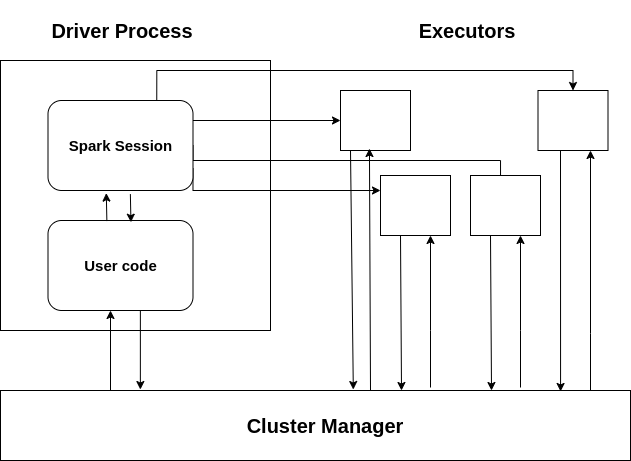
\includegraphics[width=0.5\textwidth]{cluster_spark.png}
    \caption{Aplicación de Spark}
    \label{fig:spark-app}
\end{figure}

En la figura \ref{fig:spark-app}, podemos la relación entre el \emph{driver process} y los \emph{executor processes}. En local, el \emph{driver process} y los \emph{executor processes} se ejecutan en el mismo computador como un \emph{hilo de ejecución} de la aplicación. 

Algunos puntos clave para entender Spark son:
\begin{itemize}
    \item Spark emplea un \emph{cluster manager} que administra los recursos disponibles.
    \item El \emph{driveer process} es responsable de la ejecución de la aplicación hasta que se completa la tarea.
\end{itemize}

Los \emph{executor processes}, en su mayor parte corren codigo Spark. Sin empargo, el driver puede \enquote*{conducir} diferentes lenguajes.

\subsection*{Api de lenguaje de Spark}

La Api de lenguaje de Spark hace posible que los usuarios de Spark escriban aplicaciones en diferentes lenguajes de programación, como por ejemplo, Python, Java, Scala, R, etc. EN general, Spark presenta algnos conceptos centrales en todo lenguaje, estos conceptos son traducidos internamentre a un lenguaje de programación específico que corra en el cluster. Con las apis estructuradas, se puede esperare un performance similar de todos los lenguajes. 



\end{document}

